\section{Embedded Systems Design} 


An embedded system is a microprocessor-based system
that is built to control a function or range of functions and is not designed to be
programmed by the end user in the same way that a PC is. A user can make choices
concerning functionality but cannot change the functionality of the system by
adding/replacing software. With a PC, this is exactly what a user can do: one minute
the PC is a word processor and the next it's a games machine simply by changing the
software. An embedded system is designed to perform one particular task albeit with
choices and different options.

The last point is important because it differentiates itself from the world of the PC
where the end user does reprogram it whenever a different software package is bought
and run. However, PCs have provided an easily accessible source of hardware and
software for embedded systems and it should be no surprise that they form the basis
of many embedded systems.

\section{Printed Circuit Board} 

Printed Circuit Boards (PCBs) are thin, rigid, and usually rectangular, with
components attached to one or both surfaces. The top and bottom are generally
coloured in dark blue or green. Lines running between the components have a slightly
different colour. In addition to the top and bottom sides, modern circuit boards have
internal planes called layers. Internal layers don’t have components but may contain
metal lines that carry electricity to and from the components on the top and bottom.
For example, the circuit board in the iPhone 4 handset has 10 layers. Layers are
critically important in PCB design, so circuit boards are commonly divided into three
categories: single-sided, double-sided, or multilayer. 

\begin{figure}[p]
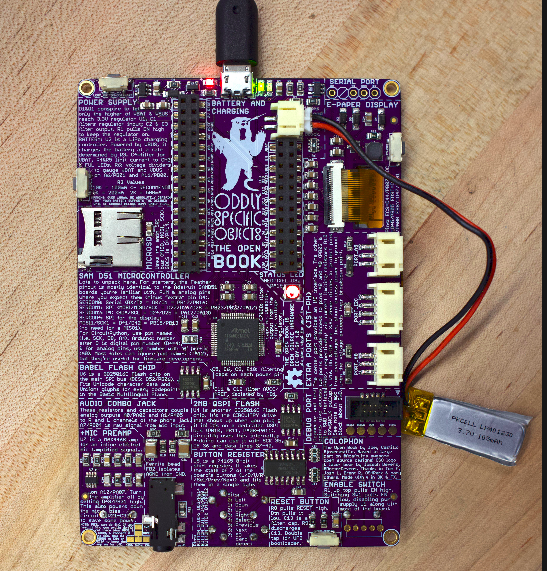
\includegraphics[width=8cm]{pcb_picture}
\centering
\caption{A Populated Printed Circuit Board.}
\centering
\label{fig:pcb_pop}


\end{figure}

\begin{figure}[p]

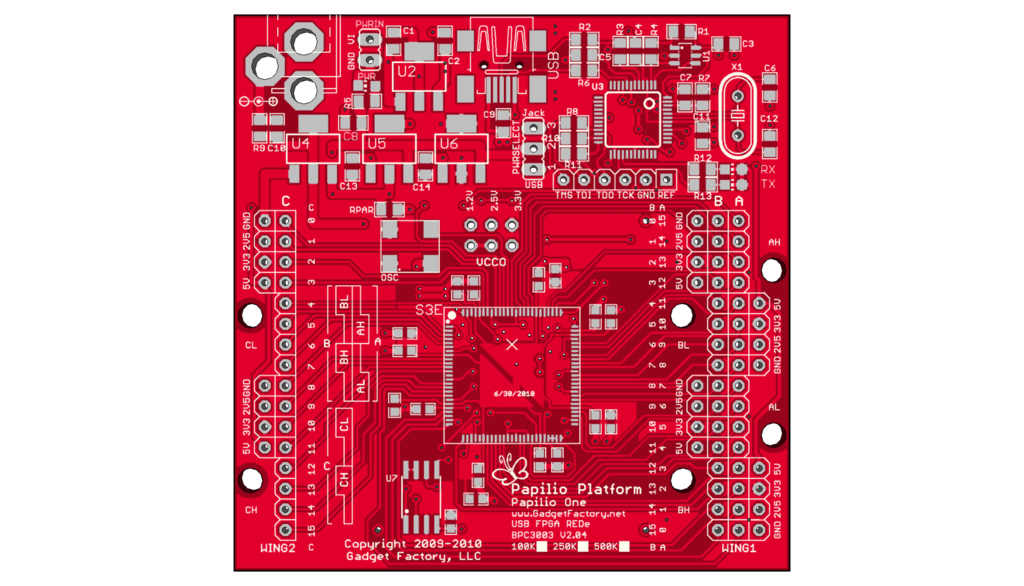
\includegraphics[width=15cm]{pcb_unpopulated}
\centering
\caption{An Unpopulated Printed Circuit Board.}
\centering
\label{fig:pcb_unpop}


\end{figure}

At the very least, a circuit board serves two purposes:
\begin{enumerate}
\item Provides mechanical support for a set of components
\item Provides electrical connections between the components
\end{enumerate}

A picture of an populated and unpopulated Printed Circuit Board are shown in Figures \ref{fig:pcb_pop} and \ref{fig:pcb_unpop} respectively. 

\section{Electrical Components}

An electronic component is any basic discrete device or physical entity in an electronic system used to affect electrons or their associated fields. Electronic components are mostly industrial products, available in a singular form and are not to be confused with electrical elements, which are conceptual abstractions representing idealized electronic components.

Electronic components have a number of electrical terminals or leads. These leads connect to other electrical components, often over wire, to create an electronic circuit with a particular function (for example an amplifier, radio receiver, or oscillator). Basic electronic components may be packaged discretely, as arrays or networks of like components, or integrated inside of packages such as semiconductor integrated circuits, hybrid integrated circuits, or thick film devices. The following list of electronic components focuses on the discrete version of these components, treating such packages as components in their own right. 

Components can be classified as passive, active, or electromechanic. The definitions of each class of electrical components are as follows
\begin{enumerate}
\item \textbf{Active :} These class of electrical components rely on a source of energy to function and usually can inject power into a circuit. Active components include amplifying components such as transistors, triode vacuum tubes (valves), and tunnel diodes.
\item \textbf{Passive :} These class of electrical components can't introduce net energy into the circuit. They also can't rely on a source of power, except for what is available from the  circuit they are connected to. As a consequence they can't amplify (increase the power of a signal), although they may increase a voltage or current (such as is done by a transformer or resonant circuit). Passive components include two-terminal components such as resistors, capacitors, inductors, and transformers.
\item \textbf{Electromechanic :}  can carry out electrical operations by using moving parts or by using electrical connections
\end{enumerate}

A lead  is an electrical connection consisting of a length of wire or a metal pad that is designed to connect two locations electrically. Electrical Components are available in three popular forms or technology. This form differ from one another by the form of their leads and method of mounting the Components. They include:



\begin{figure}[p]
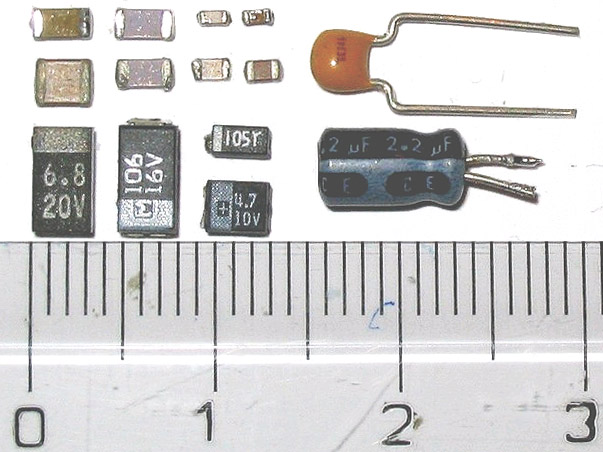
\includegraphics[width=8cm]{Photo-SMDcapacitors}
\centering
\caption{A collection of SMD Components.}
\centering
\label{fig:smd1}


\end{figure}

\begin{figure}[p]

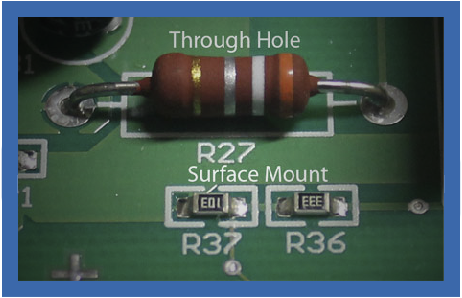
\includegraphics[width=15cm]{THT_SMD}
\centering
\caption{A board containing THT and SMD Components.}
\centering
\label{fig:THT_SMD}


\end{figure}
\begin{enumerate}
\item \textbf{Through Hole Technology:} This refers to the mounting scheme used for electronic components that involves the use of leads on the components that are inserted into holes drilled in printed circuit boards (PCB) and soldered to pads on the opposite side either by manual assembly (hand placement) or by the use of automated insertion mount machines. It is the oldest form of electrical components and is fast becoming obsolete with improving technology.
\item \textbf{Surface-mount technology (SMT):} is a method for producing electronic circuits in which the components are mounted or placed directly onto the surface of printed circuit boards (PCBs). An electronic device so made is called a surface-mount device (SMD). In industry, it has largely replaced the through-hole technology construction method of fitting components with wire leads into holes in the circuit board. Both technologies can be used on the same board, with the through-hole technology used for components not suitable for surface mounting such as large transformers and heat-sinked power semiconductors. An SMT component is usually smaller than its through-hole counterpart because it has either smaller leads or no leads at all. It may have short pins or leads of various styles, flat contacts, a matrix of solder balls (BGAs), or terminations on the body of the component. 
\end{enumerate}


\section{LoRa (Long Range)}
LoRa (\textbf{Lo}ng \textbf{Ra}nge) is a low-power wide-area network (LPWAN) technology. It is based on spread spectrum modulation techniques derived from chirp spread spectrum (CSS) technology.[1]It was developed by Cycleo of Grenoble, France and acquired by Semtech, the founding member of the LoRa Alliance.
Semtech’s LoRa devices and wireless radio frequency technology is a long range, low power wireless platform that has become the de facto technology for Internet of Things (IoT) networks worldwide.

LoRa uses license-free sub-gigahertz radio frequency bands like 433 MHz(Nigeria), 868 MHz (Europe) and 915 MHz (Australia and North America). LoRa enables long-range transmissions (more than 10 km in rural areas) with low power consumption. The technology covers the physical layer, while other technologies and protocols such as LoRaWAN (Long Range Wide Area Network) cover the upper layers. 

Semtech’s LoRa devices have amassed several hundred known uses cases for smart cities, smart homes and buildings, smart agriculture, smart metering, smart supply chain and logistics, and more. The technology can be utilized by public, private or hybrid networks and provides greater range than Cellular networks. LoRa Technology can easily plug into existing infrastructure and enables low-cost battery-operated IoT applications. The figur \ref{fig:lo1} shows how Lora compares to conventional form of data transmission. 

\subsection{Chirp Spread Spectrum (CSS)}
Chirp Spread Spectrum (CSS) is a spread spectrum technique that uses wideband linear frequency modulated chirp pulses to encode information.[1] A chirp is a sinusoidal signal of frequency increase or decrease over time (often with a polynomial expression for the relationship between time and frequency). In \ref{fig:css} is an example of an upchirp in which the frequency increases linearly over time. Sometimes the frequency of upchirps increase exponentially over time. 

As with other spread spectrum methods, chirp spread spectrum uses its entire allocated bandwidth to broadcast a signal, making it robust to channel noise. Further, because the chirps utilize a broad band of the spectrum, chirp spread spectrum is also resistant to multi-path fading even when operating at very low power. However, it is unlike direct-sequence spread spectrum (DSSS) or frequency-hopping spread spectrum (FHSS) in that it does not add any pseudo-random elements to the signal to help distinguish it from noise on the channel, instead relying on the linear nature of the chirp pulse. Additionally, chirp spread spectrum is resistant to the Doppler effect, which is typical in mobile radio applications.

Chirp spread spectrum was originally designed to compete with ultra-wideband for precision ranging and low-rate wireless networks in the 2.45 GHz band. However, since the release of IEEE 802.15.4a (also known as IEEE 802.15.4a-2007), it is no longer actively being considered by the IEEE for standardization in the area of precision ranging.

\begin{figure}[p]
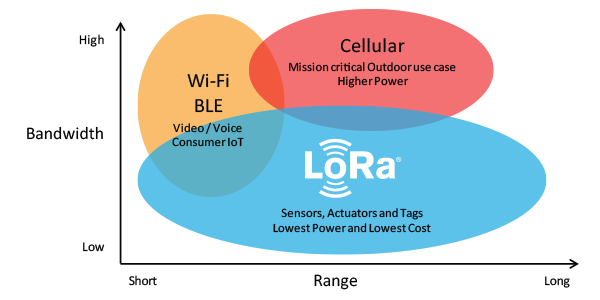
\includegraphics[scale = 0.7]{LoRa_Why_Range}
\centering
\caption{A dipiction of Lora compared to other networks.}
\centering
\label{fig:lo1}


\end{figure}

\begin{figure}[p]

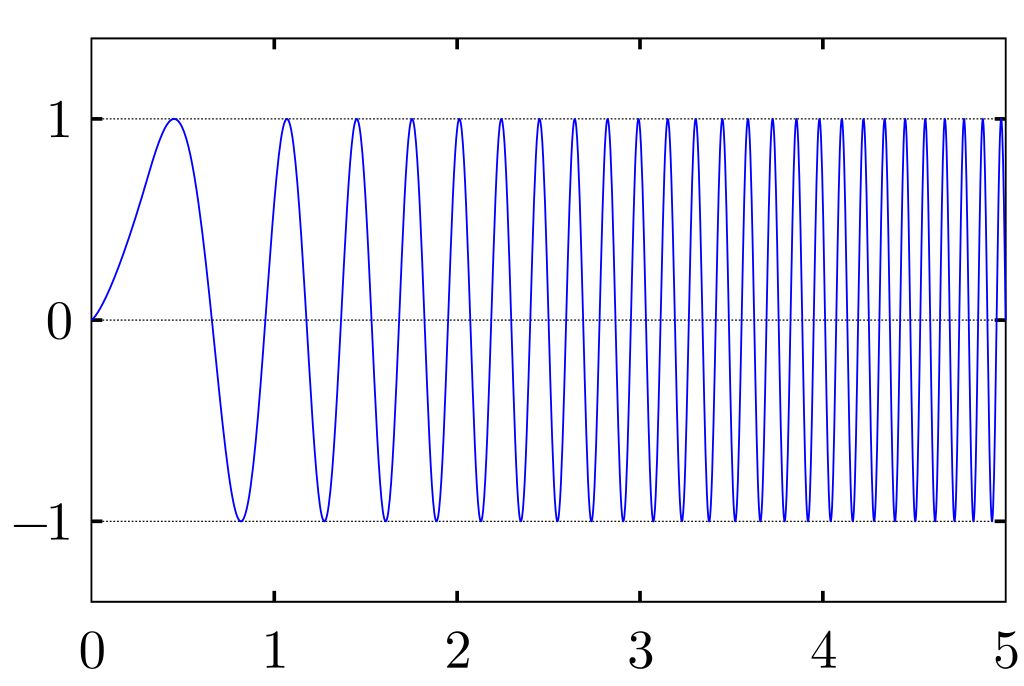
\includegraphics[width=15cm]{Linear-chirp}
\centering
\caption{A linear frequency modulated upchirp in the time domain.}
\centering
\label{fig:css}
\end{figure}

Chirp spread spectrum is ideal for applications requiring low power usage and needing relatively low data rates (1 Mbit/s or less). In particular, IEEE 802.15.4a specifies CSS as a technique for use in Low-Rate Wireless Personal Area Networks (LR-WPAN).




\subsection{Advantages of LoRa (Long Range)}
The advantages of LoRa includes the following
\begin{enumerate}
\item \textbf{Long Range :} LoRa devices are known to be able to transmit for very large distance. This makes them perfect for use in very remote and rural areas. The maximum number of distance a LoRa device can transmit depends on its power requirement and presence or absence of a Low Noise Amplifier (LNA). Commercially available Lora modules are known to transmit for up to three to eight Kilometers depending on the surrounding. 
\item \textbf{Low Power :} LoRA devices pride themselves with the abilty to last for a long time while running on batteries. This is due to their very low rate of power consumption. A Lora device requires minimal energy, with prolonged battery lifetime of up to 10 years, minimizing battery replacement costs
\item \textbf{License-free radio frequency bands :}  Lora Devices make use of radio frequency bands like 433 MHz(Nigeria), 868 MHz (Europe) and 915 MHz (Australia and North America). These frequency bands are available in everywhere and free to be used without a transmitting license. 
\item \textbf{GeoLocation :}  Enables GPS-free tracking applications, offering unique low power benefits untouched by other technologies. Lora Devices can be located by certain triangularization techniques. This means that we can know what device sent a payload and where such device is stationed. 
\end{enumerate}

\subsection{Disadvantages of LoRa (Long Range)}
The disadvantages of LoRa includes the following
\begin{enumerate}
\item \textbf{Low bit Rate :} LoRa devices are unable to transmit data with high bit rate. This is a basic trade off for Low power and long range.The maximum bit rate you’ll see is 50kpbs. This makes them useful in systems that dont require transmission of large data within a short period. An example of such system is a sensor mesh 
\item \textbf{Latency  :} Even though it is a low latency modulation it’s not low enough for applications that demand very responsive real time communications.
\end{enumerate}

